% Working document for Assignment 4. Select this file as the main file in Overleaf.
\documentclass[a4paper,11pt]{article}
\usepackage[utf8]{inputenc}
\usepackage[T1]{fontenc}
\usepackage{lmodern}
\usepackage[english]{babel}
\usepackage[a4paper,margin=25mm]{geometry}
\usepackage{microtype}
\usepackage{graphicx}
\usepackage{booktabs,tabularx}
\usepackage{amsmath,amssymb}
\usepackage{enumitem}
\usepackage[hidelinks]{hyperref}
\setlist{nosep}
\renewcommand{\thesection}{Part \arabic{section}}
\renewcommand{\thesubsection}{\arabic{section}.\arabic{subsection}}

\title{IT3212 -- Assignment 4\\Reinforcement Learning}
\author{\textit{[Author names or candidate numbers]}}
\date{\textit{[Final submission date]}}

\begin{document}
\maketitle
\noindent\textbf{Team option:} MsPacMan

% This is a combined writing document, not a claim that all submission records
% are complete. The brief separately requests predictions, an evidence brief,
% a review record, code/experiment records and an AI-assistance record.
% Evidence-brief working layout: Parts 2, 3, 4 and 6, at most 2,000 words
% excluding tables and figure captions. Part 5: review record, at most 1,000 words.
% To prepare separate documents, retain the corresponding input lines below.
% Each section sets its original Part number, so numbering survives extraction.

\section{Predictions Before Training}

%\textbf{Assumptions.} We compare tabular Q-learning using a compact, discretised set of game features with PPO using the same underlying features at a finer level of detail. Features include MsPacMan's position, nearby ghosts, pellets and power-pellet status. We define success as reaching a score of 2,000 points, which is a reasonable score to achieve upon completing the first level. Failure is defined as losing all remaining lives without reaching 2000 points. These are predictions, not results.


\textbf{Assumptions:} We compare tabular Q-learning using a compact, discretised set of game features with PPO using the same underlying features at a finer level of detail. These features include MsPacMan's position, nearby ghosts, pellets, and remaining power-pellet time. Rewards are based on the game score. We define success as reaching at least 2,000 points before losing all lives or reaching the maximum episode length. We consider 2,000 points a reasonable score to achieve by the time the first level is completed. Failure means that the agent does not reach 2,000 points before either of these limits. These are predictions, not results.


\subsection{Which agent will improve fastest with a small interaction budget?}
\textbf{Prediction:} Q-learning will improve faster at first. Provided a small interaction budget, we expect it to have a higher evaluation success rate than PPO.

\textbf{Why:} Q-learning updates the estimated value of a state--action pair after each move. If similar situations are grouped into a small number of states, it can quickly learn useful choices, such as moving away from nearby ghosts. PPO must collect experience and then update both its policy and value estimates. With little data, those updates may take longer to produce reliable behaviour. However, Q-learning's early advantage depends on the state table being small enough for important situations to be visited often.

\subsection{Which agent will show the largest performance variation across seeds?}
\textbf{Prediction:} Q-learning will show more variation in evaluation success rate across training seeds.

\textbf{Why:} MsPacMan has many possible routes, and a few early encounters with ghosts or power pellets can strongly affect what an agent learns. In a Q-table, an action that has rarely been tried may keep an inaccurate value for a long time. Different random seeds can therefore lead to very different routes. PPO also depends on random experience, but its shared model can learn from related states instead of estimating every state--action pair separately. We expect this to reduce variation, although it is not guaranteed.

\subsection{How will stochastic transitions change the routes agents learn?}
\textbf{Prediction:} When moves become less predictable, both agents will choose safer routes more often than when every action has a fixed outcome. We expect Q-learning's success rate to fall more than PPO's.

\textbf{Why:} When an action does not always produce the expected movement, a route close to a ghost becomes less reliable. A small movement error may turn a shortcut into a collision, so a longer route with more space can give a better chance of survival. Q-learning can learn this too, but its table needs enough visits to estimate the risk in each relevant state. PPO may cope better if its model learns a similar avoidance pattern across many positions. This prediction assumes the training budget is too small for Q-learning to visit every risky situation often.

\subsection{How might a penalty for each step change success rate and episode length?}
\textbf{Prediction:} We expect the effect of a step penalty to depend on its size. A small negative reward for each move may lead to shorter successful episodes without significantly reducing the success rate. However, a larger penalty may reduce the success rate by encouraging riskier routes.

\textbf{Why:} A small step penalty gives the agent a reason to reach 2,000 points with fewer moves rather than taking unnecessary detours. However, in MsPacMan, the shortest route to more points may pass close to ghosts. If the penalty is too large, the agent may prioritise speed over survival and lose all its lives before reaching the target. We therefore expect a moderate penalty to improve efficiency, but a large penalty could make the agent less reliable. 

\subsection{Will the agent with the highest training return also perform best during evaluation?}
\textbf{Prediction:} We expect the agent with the highest training return to generally perform better during evaluation, but this is not guaranteed.

\textbf{Why:} Since rewards are based on the game score, a higher training return means that the agent has collected more points during training. However, our definition of success is reaching 2,000 points, which means that a higher average score does not necessarily lead to a higher success rate. For example, an agent that consistently scores 1,900 points would have a higher average return than one that sometimes reaches 2,000 points but often scores much lower. Different ghost movements and random seeds may also affect how well the agents perform during evaluation. Therefore, we expect a positive relationship between training return and evaluation success rate, but not a perfect one.

\subsection{Which agent would you initially recommend, and what evidence would change your mind?}

\textbf{Prediction:} We would initially recommend PPO because MsPacMan has a large and complex state space involving ghosts, pellets, and changing positions.
\textbf{Why:} MsPacMan has many possible states involving ghost positions, remaining pellets, and the player's position. We expect tabular Q-learning to struggle because representing all these states would require a very large Q-table. Simplifying the state representation could reduce the table size but may remove useful information. PPO uses a neural network that can learn patterns across similar situations, which may help it make better decisions in unfamiliar states. However, PPO may require more computation and training interactions to learn effectively.

\textbf{Evidence that would change our mind:} We would reconsider our recommendation if Q-learning achieves a higher evaluation success rate than PPO with the same interaction budget. We would also consider the variation across random seeds and the time required for training. If Q-learning consistently reaches 2,000 points more often while requiring fewer resources, we would recommend it instead.

\subsection{Three states where we expect the approaches to behave differently}
For each state, we predict Q-learning's highest-value action and PPO's highest-probability action. These differences are hypotheses based on the state representations above, not properties the algorithms must always have.

\subsubsection{State 1: Ghost near a shortcut}
\textbf{State:} MsPacMan reaches a junction. Pellets are on the right, but a normal ghost is moving towards her from that direction. Going up is a longer route with more space between her and the ghost.

\textbf{Expected actions:} Q-learning: \textbf{RIGHT}. PPO: \textbf{UP}.

\textbf{Why:} A coarse Q-table may group together junctions where the ghost is close and where it is farther away. If moving right was often rewarded in those grouped states, Q-learning may still choose it here. PPO may use the finer information about the ghost's location to choose the safer route upward. This could improve its chance of surviving long enough to reach 2,000 points. The difference depends on whether the Q-table loses useful distance information.

\textbf{What would contradict this prediction:} If, when tested at this junction, Q-learning favours UP or PPO favours RIGHT, the predicted action for that agent is contradicted. If both consistently favour the same action, our predicted difference between the agents is not supported.

\subsubsection{State 2: Frightened ghost}
\textbf{State:} A frightened ghost is on the right, with pellets behind it. There is enough power time left to pass it safely. Moving up avoids the ghost but takes a longer path.

\textbf{Expected actions:} Q-learning: \textbf{UP}. PPO: \textbf{RIGHT}.

\textbf{Why:} A coarse Q-learning state may treat frightened-ghost situations alike, even when the remaining power time differs. If the agent has learned to avoid uncertain encounters, it may turn up. PPO may distinguish how much power time remains and recognise that passing the ghost is currently safe and gives access to points that help it reach the 2,000-point target. This prediction requires the power timer to be represented more precisely for PPO.

\textbf{What would contradict this prediction:} If Q-learning favours RIGHT or PPO favours UP when enough power time remains, the predicted action for that agent is contradicted. If both consistently choose the same direction, the expected difference is not supported.

\subsubsection{State 3: Only a few pellets nearby}
\textbf{State:} One pellet is nearby on the right, while a larger group of pellets is on the left. Neither direction has an immediate ghost threat, and the agent has not yet reached 2,000 points.

\textbf{Expected actions:} Q-learning: \textbf{RIGHT}. PPO: \textbf{LEFT}.

\textbf{Why:} A compact Q-learning state that mainly describes nearby pellets may favour collecting the closest one, since this gives an immediate reward. PPO may use information about the wider pellet layout and learn that moving left leads to more points with less backtracking. Both algorithms can learn to value future rewards, but PPO may have an advantage because its state representation includes more information about the maze.

\textbf{What would contradict this prediction:} If Q-learning favours LEFT or PPO favours RIGHT in this state, the predicted action for that agent is contradicted. If both consistently favour the same direction, the expected difference is not supported.

% Evidence-focused Part 2 revision, 23 November 2026.
% Preserve this editorial version when regenerating historical numerical exports.
\setcounter{section}{1}
\section{Compare learning settings}
\label{sec:learning-settings}

\subsection{Task and fair comparison}
We evaluate goal attainment in Gymnasium's native \texttt{ALE/MsPacman-v5}.
The goal is at least 2,000 newly earned points. Episodes end at the target,
game over or 1,000 decisions; reaching the target counts as success, not
level completion. The finite horizon is terminal and time remaining is
observable. One interaction is one decision,
normally four emulator frames, summed across PPO's parallel environments.
Our instructor-approved adaptation replaces the brief's terminal-only reward
with score increments in A/B. C subtracts 0.1 points per decision. Both agents
learn from rewards divided by 100; reported returns are in game points.

A uses deterministic transitions on the training maze. B changes only
frame-level sticky-action probability from zero to 0.25; C adds the penalty
to B. D freezes B's agents and uses the transfer maze, unseen during training.
These are native game mazes selected through RAM before the first action:
0 and 1 are identifiers, not difficulty ratings. The observation/action formats
remain compatible. A fixed graph supplies approximate food/corridor features;
ghost positions come from RAM and all actions remain available. Q discretises a subset of the same features that
PPO receives more finely. Table~\ref{tab:part2-configuration} gives the fixed
configurations. The power-related RAM signal is a proxy, not the precise
countdown assumed in Part~1.

Every A/B/C run consumes 262,144 interactions: 128 PPO rollouts of 2,048
transitions, chosen to fit available resources, not to establish convergence.
Training seeds 17, 29, 101, 314 and 2718 are arbitrary identifiers fixed
before training, not selected for performance. Both methods use this list;
shared seeds do not imply identical experience. The new search allowance is
equal: seven packages per method on A/B with seed 42, then the best two
repeat with seed 7, totalling 4,718,592 interactions per method. Twenty
development episodes per checkpoint select one configuration by mean A/B
success, then score and earlier checkpoint. Earlier unequal exploration
informed these candidates; this is a workflow comparison after development.

Main development checks use ten episodes at 0 and every 65,536 interactions.
The same source-setting success/score/earlier-checkpoint rule selects each
trained agent's saved policy. Selected weights contain 131,072--262,144
transitions, while costs include the full cap. D inherits B's checkpoint;
final or D outcomes never select agent configurations, checkpoints or training seeds.

Each agent has 200 frozen evaluation episodes per condition: A/B/C use seeds
1150000--1150199, D uses 1250000--1250199, separate from training and development.
These numerical ranges organise phases; large values confer no statistical
advantage. Evaluation uses greedy Q with seeded uniform ties and PPO's
highest-probability action. Updates are disabled. Parameter fingerprints and native score registers
check frozen policies and earned points. Results average five trained agents,
not 1,000 episodes treated as training replications. Deterministic A can repeat
trajectories, so more episodes do not replace more training seeds.

\subsection{Measured outcomes and resource costs}
Tables~\ref{tab:part2-outcomes} and~\ref{tab:part2-costs} use the 22 November
2026 main study for A/B/C and the 23 November 2026 frozen-transfer study for D.

\begin{table}[htbp]
\centering\small
\begin{tabular}{@{}llrr@{}}
\toprule
Setting & Agent & Success (\%) & Return \\
\midrule
A & Q-learning & $32.9 \pm 39.2$ & $1490.0 \pm 413.4$ \\
A & PPO & $80.0 \pm 44.7$ & $2056.0 \pm 167.1$ \\
B & Q-learning & $32.2 \pm 21.3$ & $1622.0 \pm 191.3$ \\
B & PPO & $67.4 \pm 18.7$ & $1909.1 \pm 157.6$ \\
C & Q-learning & $26.9 \pm 13.9$ & $1462.9 \pm 201.4$ \\
C & PPO & $52.7 \pm 32.1$ & $1806.5 \pm 299.8$ \\
D & Q-learning & $4.5 \pm 2.9\;{}^{\dagger}$ & $869.6 \pm 132.5$ \\
D & PPO & $14.7 \pm 17.1\;{}^{\dagger}$ & $1065.6 \pm 439.0$ \\
\bottomrule
\end{tabular}
\caption{Mean evaluation outcomes \(\pm\) sample SD across five training
seeds, 200 episodes per agent/condition. SD describes training variation,
not a confidence interval. Returns are game points; C includes its step
penalty. \(\dagger\) D reports verified success before map exit; censored
returns cover the last verified in-map prefix, excluding the crossing reward.}
\label{tab:part2-outcomes}
\end{table}

Failure rates for Q/PPO are 67.1\%/20.0\% in A, 67.8\%/32.6\% in B and
73.1\%/47.3\% in C. D known-failure rates are 95.4\%/85.3\%, with one
censored Q episode and none for PPO among 1,000 episodes per method.
Success, known failure and censoring partition outcomes; censoring is not
silently classified as failure.

\begin{table}[htbp]
\centering\small\setlength{\tabcolsep}{3pt}
\begin{tabular}{@{}llrrrr@{}}
\toprule
Setting & Agent & Success length & Failure length & Train (s) & Evaluate (s) \\
\midrule
A & Q-learning & $521 \pm 226$ & $707 \pm 103$ & $729.9 \pm 17.3$ & $328.7 \pm 88.2$ \\
A & PPO & $513 \pm 122$ & $851$ & $602.2 \pm 3.4$ & $524.0 \pm 155.1$ \\
B & Q-learning & $655 \pm 84$ & $761 \pm 13$ & $824.6 \pm 180.4$ & $386.5 \pm 38.2$ \\
B & PPO & $578 \pm 73$ & $913 \pm 37$ & $662.3 \pm 78.4$ & $533.2 \pm 132.4$ \\
C & Q-learning & $625 \pm 58$ & $758 \pm 23$ & $1168.1 \pm 14.1$ & $326.8 \pm 18.3$ \\
C & PPO & $533 \pm 167$ & $900 \pm 7$ & $752.0 \pm 2.9$ & $373.2 \pm 99.8$ \\
D & Q-learning & $746 \pm 37$ & $582 \pm 13$ & $0$ & $215.0 \pm 24.3$ \\
D & PPO & $763 \pm 75$ & $749 \pm 111$ & $0$ & $243.7 \pm 30.4$ \\
\bottomrule
\end{tabular}
\caption{Same source studies as Table~\ref{tab:part2-outcomes}. Lengths are
per-agent mean decisions conditional on outcome, then mean \(\pm\) sample SD
across agents with that outcome. A/PPO failure length represents one agent;
D failure lengths exclude censoring. Training covers the full 262,144
interactions, excluding development checks and tuning. Evaluation covers 200
episodes, trace collection and native checks, excluding model loading and
trace compression. D incurs zero training.}
\label{tab:part2-costs}
\end{table}

Runs use an Intel Core Ultra 7 258V CPU on Windows 11, one numerical thread
per worker, up to eight workers per phase and sixteen during main-training/
evaluation overlap. Equal interactions do not imply equal computation;
shared-compute timings cannot establish an isolated algorithm speed advantage.

\begin{table}[htbp]
\centering\small
\begin{tabularx}{\linewidth}{@{}lXX@{}}
\toprule
Component & Q-learning & PPO \\
\midrule
Learning rule & Off-policy, one table; one Bellman update per real transition;
terminal targets do not bootstrap & On-policy, clipped actor--critic \\
Learning rate & 0.15 & Linear $0.0003\to0.00005$ \\
Discount & 0.995 & 0.995 \\
Training exploration & Epsilon $1\to0.05$ over first 80\% of the cap,
then 0.05 & Linear entropy coefficient $0.02\to0.002$ \\
Data/update & One new transition per update & Four 512-step environments;
batch 256; up to six epochs per rollout \\
PPO stabilisation & -- & GAE 0.97; clip 0.15; target KL 0.015 \\
Representation/model & Food-relative discrete key & 23 inputs per action,
shared two-layer 32-unit tanh scorer; separate 49-input, two-layer 64-unit critic \\
\bottomrule
\end{tabularx}
\caption{Selected configurations, held fixed across A/B/C; D reuses B.
Both receive the same 61-value observation format. The selected agents use
the 49-value prefix, with Q discretising a subset; twelve additional channels
are unused. Software: Gymnasium 1.4.0, ALE 0.12.1, PyTorch 2.14.1,
Stable-Baselines3 2.9.2 and Python 3.13.7.}
\label{tab:part2-configuration}
\end{table}

\begin{figure}[htbp]
\centering
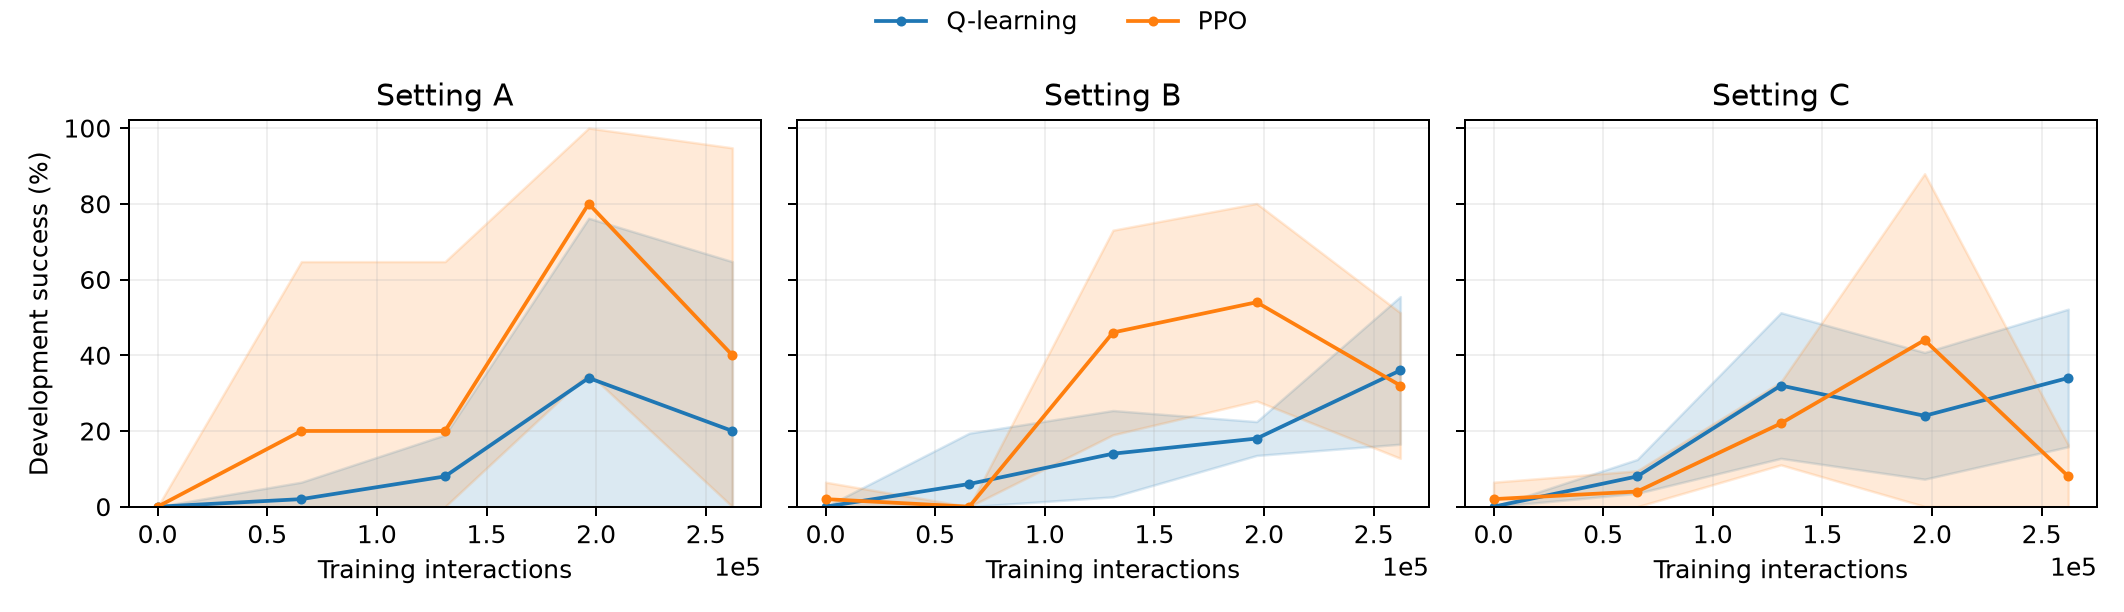
\includegraphics[width=\linewidth]{Images/part2_learning_curves_20261122.png}
\caption{Source: 22 November 2026 main experiment, training seeds 17/29/101/314/2718,
settings A/B/C and Table~\ref{tab:part2-configuration}'s configurations.
Unsmoothed mean development success, checked on ten episodes per agent at
0 and every 65,536 interactions; shading is one sample SD across five agents,
clipped to 0--100\%, not a confidence interval. Final tests are excluded.
Table~\ref{tab:part2-outcomes} evaluates development-selected checkpoints,
which can precede the curves' last point.}
\label{fig:part2-learning}
\end{figure}

\setcounter{section}{2}
\section{Investigate the mechanisms}
\label{sec:mechanisms}

\subsection{Controlled comparisons}
% State all tested values and what remains fixed; change one main factor at a time.
% Use at least FIVE training seeds for EVERY tested configuration.
% Cover Q-learning epsilon schedules, discount factors, PPO entropy coefficients,
% learning rates and PPO update epochs per rollout. Explain the mechanism each
% comparison probes. Report observed effects with source configuration/run IDs.
\noindent\textit{[Describe the controlled experiments and their measured results.]}

\subsection{Revisit predictions and test an explanation}
% Reference the untouched Part 1 predictions. State support/contradiction, inspect
% a case that does not fit the explanation, and offer a plausible competitor.
% Describe one small diagnostic that distinguishes the explanations: question,
% controlled change, source runs, observation and what can/cannot be concluded.
% A larger training budget alone is insufficient unless it tests the explanation.
\noindent\textit{[Connect observations to the original predictions and diagnostic evidence.]}

\setcounter{section}{3}
\section{Inspect what aggregate scores hide}
\label{sec:episodes}

\subsection{Episode selection}
% Select ten RECORDED episodes: 3 typical successes, 3 typical failures,
% 2 surprising successes and 2 surprising failures. Justify typicality using
% the outcome distributions and explain the surprise criterion before interpretation.
% Record episode ID, source run/configuration, setting, agent and evaluation seed.
\noindent\textit{[Identify the ten episodes and justify their selection.]}

\subsection{Three important decisions per episode}
% Annotate THREE decisions in EACH of the ten selected episodes (30 in total).
% For each decision include: state and available actions; chosen action and actual
% Q-values or policy probabilities; observed transition and outcome; alternative
% action, what might have happened, and what remains uncertain.
% Use compact inline tables or trace figures with source run/episode/step IDs.
% Do not invent counterfactual transitions or probabilities absent from the traces.
\noindent\textit{[Insert the recorded decision annotations.]}

\subsection{What aggregate results miss}
% Use specific inspected episodes to distinguish poor decisions from unlucky
% transitions and explain at least one limitation of the aggregate scores.
\noindent\textit{[Explain the limitation using episode evidence.]}

\setcounter{section}{4}
\section{Conduct a human review}
\label{sec:human-review}

\noindent\textbf{Review record:} Team review (Fredrik, Johan, Elling and Mats), 26 November 2026,
examining unified Part~2 A--D runs (\texttt{affae3e137cbe226}, \texttt{e8c0c6a8f4071325},
\texttt{9e25203dcd939450}, \texttt{unified\_part2/setting\_D}), Part~3 sweeps and diagnostics
(\texttt{054b0e6b63381969}, \texttt{3142fac3111db314}, \texttt{exec\_diagnostic}) and Part~4 replays.

\subsection*{Strongest supporting evidence}
The strongest evidence for preferring PPO in uncertain simulation is the matched Setting~B
comparison executed in one consistent computing environment: baseline PPO achieved 70.2\%
mean success against Q-learning's 31.3\% across five training seeds and 200 frozen episodes
per model, outperforming Q on all five paired seeds. In Part~3's locked confirmation on the
same 200 test seeds, PPO12 ($2\times$ learning rate, 12 epochs) raised mean success further
to 90.2\% while halving between-seed SD from 16.1 to 8.0 percentage points. Because Q and PPO
use different state encodings from the shared observation vector, this supports the tested
workflows rather than PPO in isolation.

The paired Setting~D study provides the cleanest control of observation sensitivity: the exact
same frozen Setting~B checkpoints ran on 200 paired seeds under clean and 32$\times$32 obstructed
observations with native dynamics untouched. Success fell from 70.2\% to 47.5\% for baseline PPO,
from 91.1\% to 70.1\% for PPO12, and from 27.1\% to 22.2\% for Q. Higher retained success and
smaller absolute degradation are distinct criteria, and opposite individual-seed shifts (e.g.,
PPO seed~2718 gaining $+8.0$ pp while seed~314 lost $-37.0$ pp) prevent universal claims.

\subsection*{A claim that goes beyond the evidence}
A tempting overstatement from the 90.2\% PPO12 score is ``PPO12 generalises reliably to
unfamiliar operating conditions.'' That claim exceeds our evidence: even under a single
fixed 32$\times$32 object-feature obstruction with intact maze geometry, PPO12 dropped 21.0
percentage points and failed 29.9\% of episodes (and baseline PPO failed 52.5\%). A defensible
statement is: the tested PPO workflows retain higher mean success than Q under this fixed local
obstruction, without establishing pixel-perception robustness, unseen-map transfer or deployment safety.

\subsection*{A competing explanation}
Two mechanisms required distinguishing competing explanations. First, PPO12's early lead at
65,536 interactions could have reflected noise from 10 development episodes; our 50-episode
fresh diagnostic (\texttt{3142fac3111db314}) ruled out pure episode noise (29.6\% for 12-epoch
PPO vs.\ 5.6\% for Q and 0\% for 6-epoch PPO), showing rollout reuse drives the early reversal.
Second, zero-entropy PPO's cap-level gain (64\% vs.\ 36\% on development) could reflect argmax
concentration rather than a uniformly superior policy distribution. On 50 fresh paired episodes,
the zero-entropy advantage narrowed from $+20.0$ pp under argmax (66.4\% vs.\ 46.4\%) to
$+14.0$ pp under sampling (57.2\% vs.\ 43.2\%), with lower action entropy (0.426 vs.\ 0.624 nats).
Thus execution mode accounts for part—but not all—of the cap-level gain, while seed~2718 still
reversed under argmax.

\subsection*{Comparison with submitted predictions}
Original Part~1 predictions remain unchanged with dated annotations attached. The predicted early
Q advantage held against 6-epoch PPO in B but was reversed by 12-epoch PPO and in A. Larger Q
seed variation held in B but not in A or C. Stochasticity lowered mean PPO success ($-9.8$ pp)
while leaving Q's mean unchanged (masking paired swings from $-73$ to $+44$ pp), and the common-pool
ghost probe showed only a 1.9 pp A-to-B PPO shift, leaving safer routes unestablished. Setting~C
shortened wins but reduced mean success and widened PPO SD. Same-state probes failed to support
State~1, could not verify State~2's precise-timer premise, and directly contradicted State~3
(PPO chose RIGHT 98.7\%, not LEFT). Accordingly, our initial preference for PPO becomes strictly
conditional on simulation use.

\subsection*{Initial priority rankings and group negotiation}
Table~\ref{tab:priorities} records each member's initial ranking of failure avoidance (F),
robustness to change (R), explainability (E) and time efficiency (T).

\begin{table}[H]\centering\small
\begin{tabular}{ll}\toprule
Member & Initial priority order\\\midrule
Fredrik & $F>R>E>T$\\
Johan   & $R>F>T>E$\\
Elling  & $F>E>R>T$\\
Mats    & $F>R>T>E$\\
\bottomrule\end{tabular}
\caption{Initial priority rankings reported by each team member before negotiation.}
\label{tab:priorities}
\end{table}

The negotiated final order was $F>R>E>T$. Three members placed failure avoidance first; Johan
initially ranked robustness first because of incomplete observations, weighing the paired D
degradation heavily ($-22.7$ pp for baseline PPO, $-21.0$ pp for PPO12). Keeping $F$ and $R$
above $E$ and $T$ reflected the group's consensus on avoiding failures under change. Fredrik and
Elling ranked explainability above time efficiency, whereas Johan and Mats ranked time efficiency
higher. We broke this tie using failure avoidance: in Part~4, 11 of 12 collision alternatives
still lost a life within 64 decisions (e.g., SF2/491 and TF2/756), and only TF2/941 avoided loss.
Being able to inspect whether an intervention actually prevents failure mattered more than minor
runtime savings, placing $E$ third and $T$ fourth. This ordering anchors Part~6: PPO12 is best for
further B simulation, but neither workflow is adequately supported for consequential autonomous
operation or unfamiliar environments.

\setcounter{section}{5}
\section{Make three recommendations}
\label{sec:recommendations}

\paragraph{Rapid classroom demonstration.}
Use Setting~B Q-learning ($\alpha=.15$, $\gamma=.995$, $\epsilon_{\mathrm{end}}=.05$) with a
prepared replay. Evidence: (1) Q trains in 3.8\,min ($225.5\pm 17.9$\,s) and led 6-epoch PPO at
65,536 steps (5.6\% vs.\ 0\%, \texttt{3142fac3111db314}); (2) table entries directly explain
choices (TS1/166: NOOP 0.79 vs.\ LEFT 0.00, +200; TS1/437: near-zero pinch values). Weakness:
68.7\% failure rate. Switch to frozen PPO12 (90.2\%) if live target completion takes priority.
Before non-simulation classroom use, pilot whether students accurately explain Q-value ties on
unseen replays.

\paragraph{Repeated operation in uncertainty.}
Recommend \emph{neither} workflow for consequential autonomous deployment; for further B
simulation, use Part~3's \textbf{PPO12} ($2\times$ LR, 12 epochs) without C's penalty. Evidence:
(1) PPO12 achieved $90.2\pm 8.0\%$ success (9.8\% failure) vs.\ 70.2\% baseline PPO and 31.3\% Q
(Table~\ref{tab:part3-heldout}); (2) C's penalty cut baseline PPO by 3.6\,pp and widened SD to
26.3\,pp, opposing $F>R>E>T$. Weakness: the weakest PPO12 seed still failed 22.5\% of episodes,
and SF2 failed at 1,990 points. Reverse only when fresh retrainings stay within a prespecified
failure bound. Before deployment, test controlled action latencies, hazard severity and human
overrides on a hardware-in-the-loop testbed.

\paragraph{Operation after an environment change.}
Recommend \emph{neither} workflow for unfamiliar conditions. Evidence: (1) under D's fixed
32$\times$32 obstruction, baseline PPO fell 22.7\,pp ($70.2\%\to 47.5\%$) and PPO12 fell 21.0\,pp
($91.1\%\to 70.1\%$, 29.9\% failure); (2) Q dropped less ($-4.9$\,pp) but still failed 77.8\%
(Table~\ref{tab:robustness-pairs}). Weakness: one small blind spot unpredictably redirects seeds.
Reverse only if locked policies meet required reliability across multiple independent shifts.
Before transfer, test unseen obstruction locations, variable dropout durations and pixel
perception on a protected testbed.

\paragraph{Scope and broader principles.}
Results reflect RAM-derived features, sticky dynamics and a 262,144-step cap, not universal
algorithm superiority. Broader principles illustrated are that directional function approximation
scales better than coarse tabular aliasing, rollout reuse governs PPO's early sample efficiency,
and high source-domain success does not certify observation robustness.


\clearpage
\section*{Consequential AI assistance record}
\textbf{18--23 November 2026.} Codex assisted with experimental design,
Gymnasium wrappers, ordinary tabular Q-learning, PPO, experiment runners,
debugging, evidence analysis and report drafting. The team authorised score
increment rewards after instructor clarification, requested ordinary Q
consistent with the original predictions, and rejected DQN. Double Q/replay
exploration was not accepted as the ordinary-Q baseline. Historical pilot
outcomes and failed candidates remain distinct from the assessed study.

Codex proposed the bounded interaction cap, relative features, matched
development search and source-only checkpoint selection. Verification checked
one Q update per transition, terminal targets, native action mapping, frozen
parameter hashes, native BCD scores and directly replayed recorded actions.
The imperfect power proxy and representation differences remain disclosed.

On 23 November Codex read both briefs, replaced primary D with a fixed
object-feature occlusion analogue, and implemented 45 fresh same-host,
five-seed one-factor models plus a frozen execution-mode diagnostic. Native
parity/noninterference checks verified D leaves the game unchanged. Original
and fresh full-budget baseline weights were compared bitwise rather than
attributing checkpoint differences to hardware or library versions.

Codex selected episodes by documented outcome distributions, reproduced 30
decision alternatives through complete seeded action prefixes, and generated
tables/figures from measured records. Snapshot restoration alone failed a
sticky-action continuation check and was rejected. One-step alternatives are
not claimed as expected-return estimates. Report checks cover numerical
provenance, original-prediction checksum, word limit, LaTeX compilation and
rendered layout.

The team requested that the actual human review be deferred. No discussion,
reviewer feedback or individual ranking was generated as human evidence.
The final prose and recommendations are AI-assisted drafts requiring the
authors' ownership and review. This record does not claim they have already
approved every conclusion or completed the outstanding human review.

\end{document}
